\section{Introducción}

\subsection{Marco contextual}

\begin{frame}{Caja}
   \begin{Block}{Arquitectura de computadoras}
      Disciplina que se encarga de determinar del comportamiento funcional de una computadora desde el punto de vista del programador. Aspectos considerados en esta disciplina son:
   \begin{itemize}
      \item Los tipos de datos y su tamaño
      \item Las operaciones que realiza
   \end{itemize}
   \end{Block}
\end{frame}

\begin{frame}{Dos columnas}
\begin{columns}
   \begin{column}{0.48\textwidth}
      \begin{itemize}
         \item item
         \item item
      \end{itemize}
   \end{column}
   \hfill
   \begin{column}{0.48\textwidth}
      \begin{AlertBlock}{alerta}
         ¡Gosh!
      \end{AlertBlock}
   \end{column}
\end{columns}
\end{frame}

\begin{frame}{Dos columnas}
   \begin{columns}
      \begin{column}{0.48\textwidth}
         \begin{itemize}
            \item item
            \item item
         \end{itemize}
      \end{column}
      \hfill
      \begin{column}{0.48\textwidth}
         \centering
         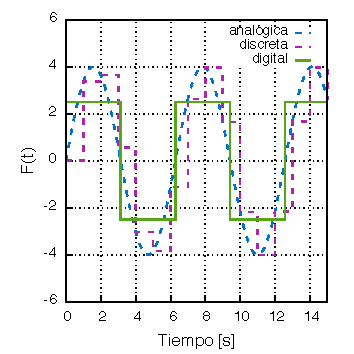
\includegraphics[width = \textwidth]{analog}
      \end{column}
   \end{columns}
\end{frame}

